\documentclass{article}
\usepackage[utf8]{inputenc}
\usepackage[spanish]{babel} 


\usepackage{graphicx} %paquete básico para incluir gráficos
\usepackage{wrapfig} %paquete Wrapfig
\usepackage{float} % paquete para controlar entornos flotantes
\usepackage{pdfpages}% Paquete pdfpages incluye páginas completas de ficheros pdfs
\usepackage{lipsum} % Paquete para introducir texto 
%
\usepackage{tikz} % Paquete TikZ para generar gráficos
\usetikzlibrary{babel,shapes,arrows}


\title{Taller LaTeX Yosigopublicando: Graficos}
\author{ossanche }
\date{March 2021}

\begin{document}

\maketitle

\section{Inclusión de gráficos}

%%%%%%%%%%%%%%%%%%%%%%%%%%%%%%%%%%%%%%%%
\lipsum % incluimos texto
{\bf Final lipsum 1}

\begin{figure}[h]
    \centering
    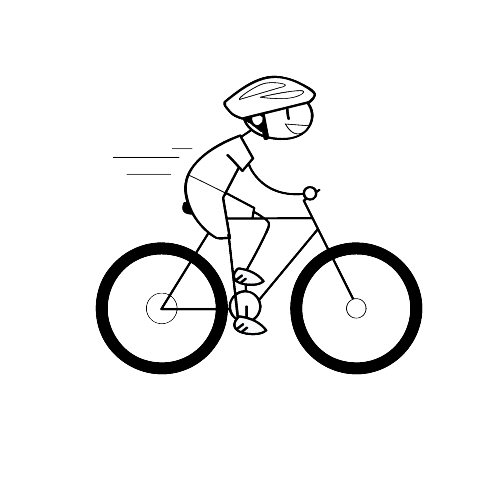
\includegraphics[height=5cm,angle=30]{graficos/ciclista.jpeg}
    \caption{Gráfico simple insertado. \LaTeX lo coloca donde estima oportuno.}
    \label{fig:1}
\end{figure}

Así esta figura puede ser referenciada haciendo una llamada a su etiqueta como se puede apreciar en Figura \ref{fig:1}.

%%%%%%%%%%%%%%%%%%%%%%%%%%%%%%%%%%%%%%%%
\lipsum % incluimos texto
{\bf Final lipsum 2}

\begin{figure}[h]
    \centering
    \frame{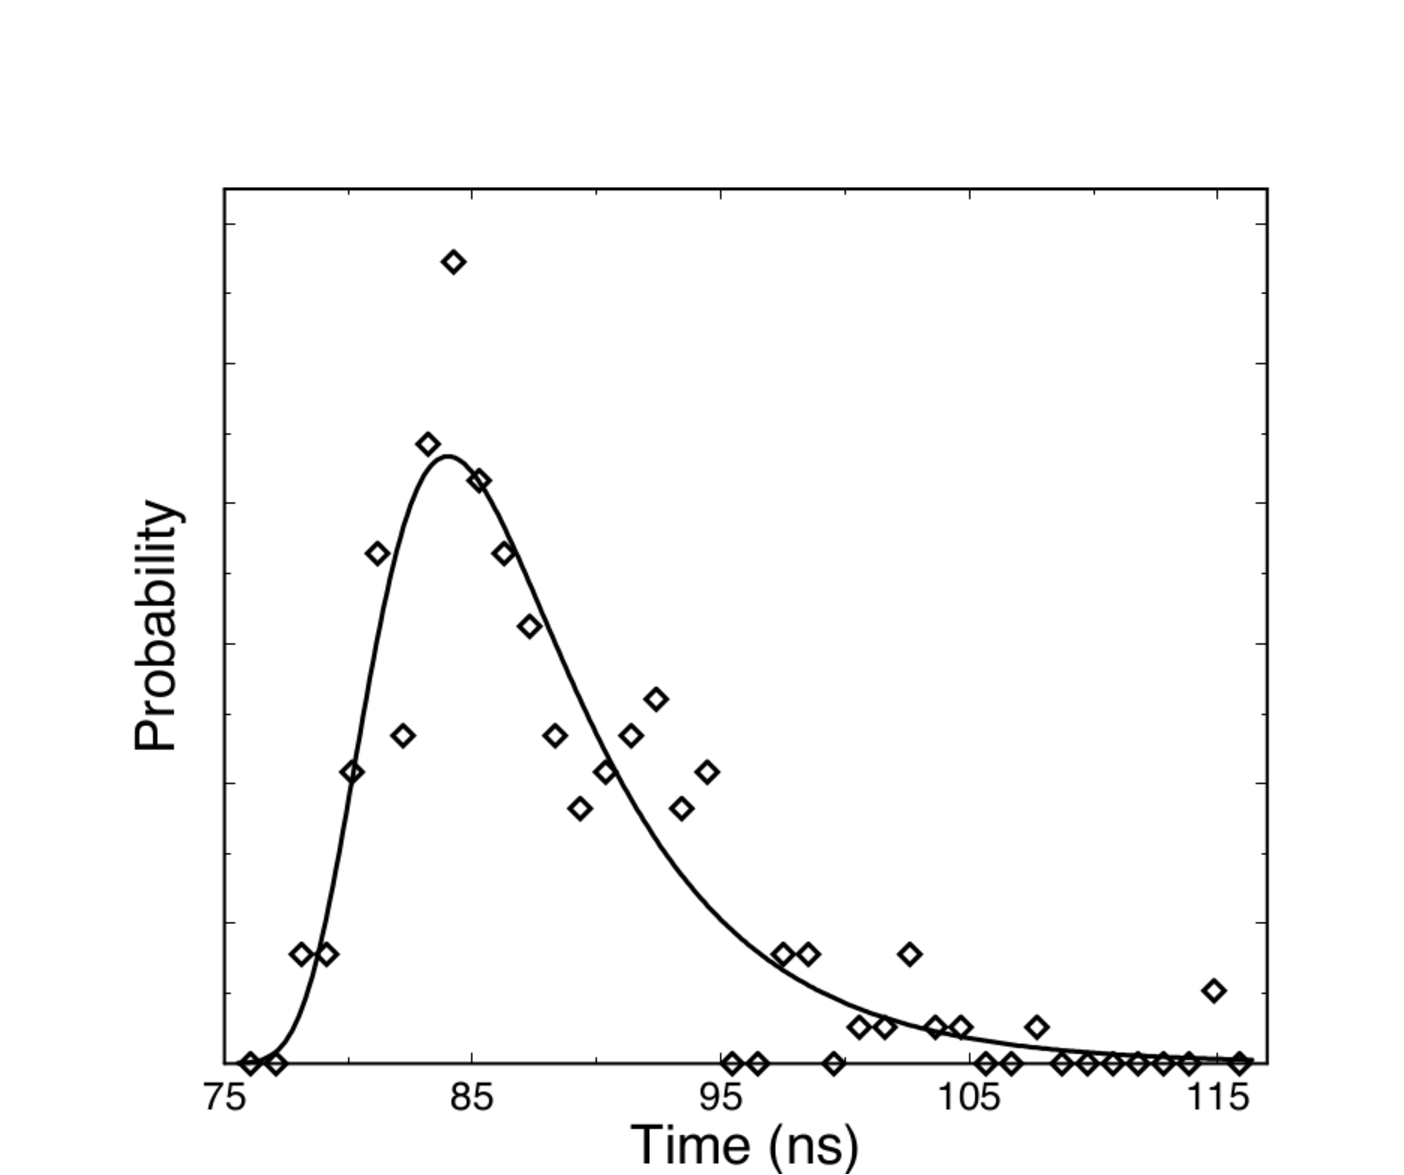
\includegraphics[width=0.45\textwidth]{graficos/fig_9Vis.pdf}}
    \frame{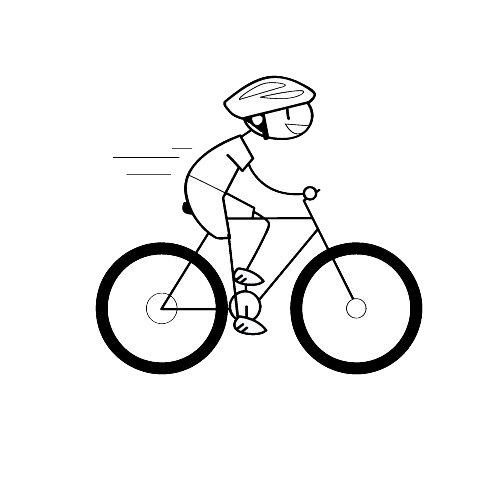
\includegraphics[width=0.45\textwidth]{graficos/ciclista.png}}
    \caption{Dos figuras contiguas. Las incluimos en un marco para poder mejorar su aspecto.}
    \label{fig:2}
\end{figure}


%%%%%%%%%%%%%%%%%%%%%%%%%%%%%%%%%%%%%%%
\lipsum

{\bf Final lipsum 3}

\begin{figure}
    \centering
    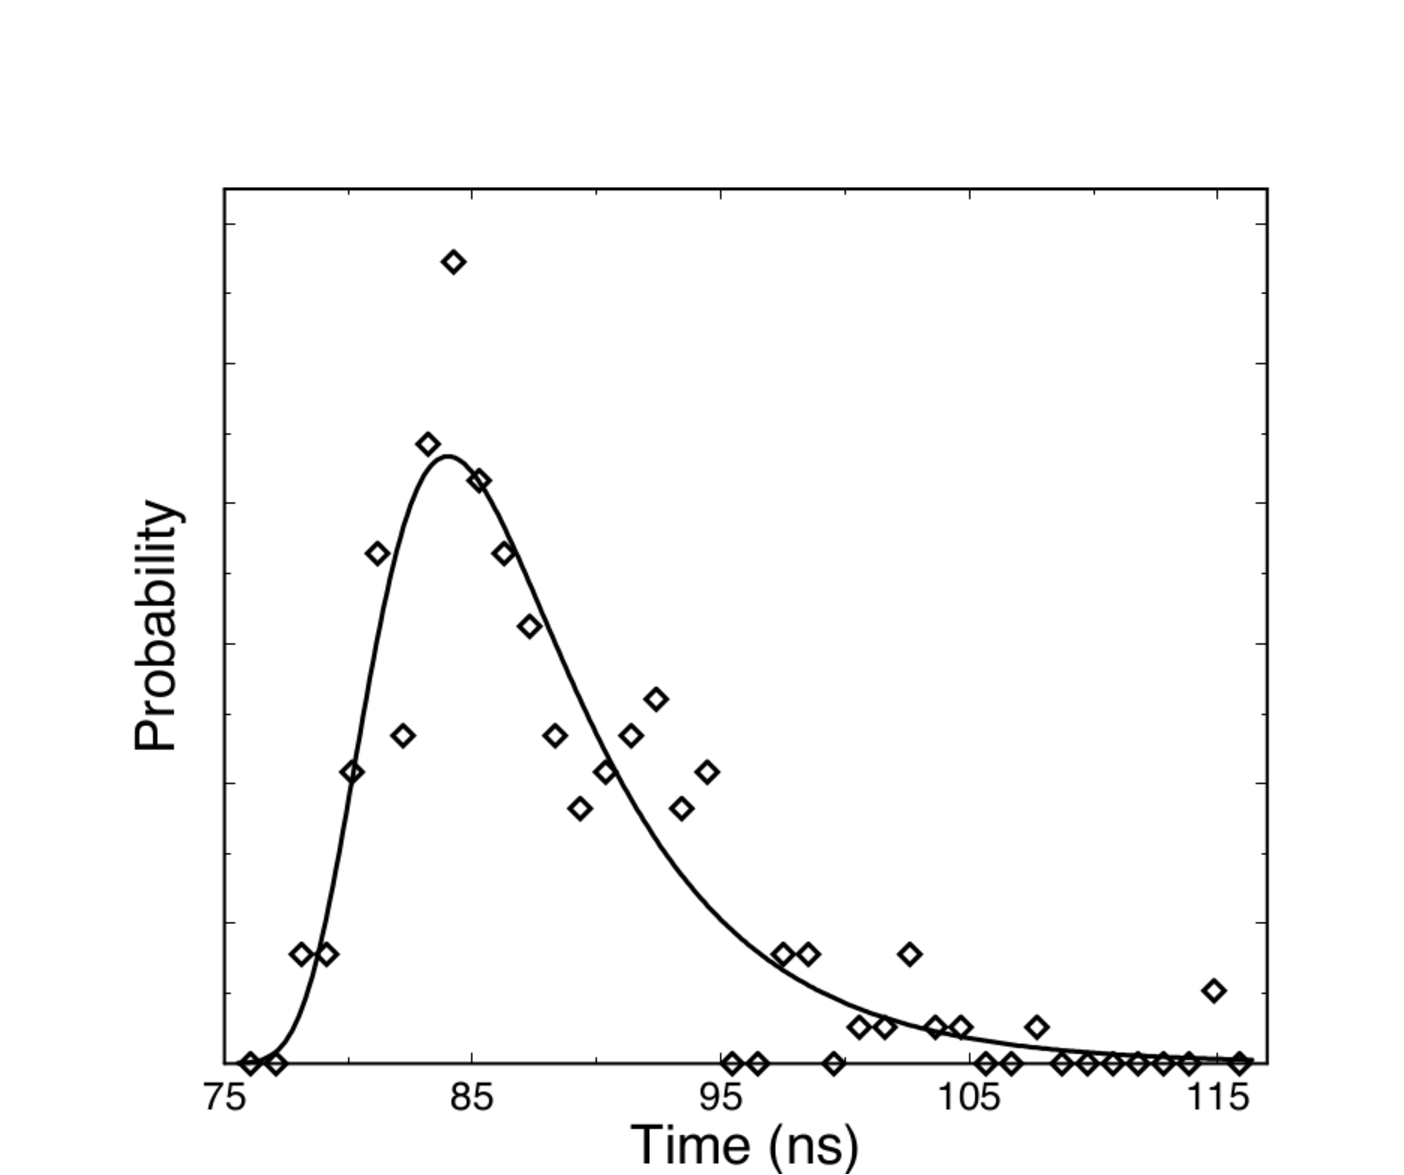
\includegraphics[trim= 0mm 0mm 0mm 30mm,clip,angle=0,width=0.45\textwidth]{graficos/fig_9Vis.pdf}
    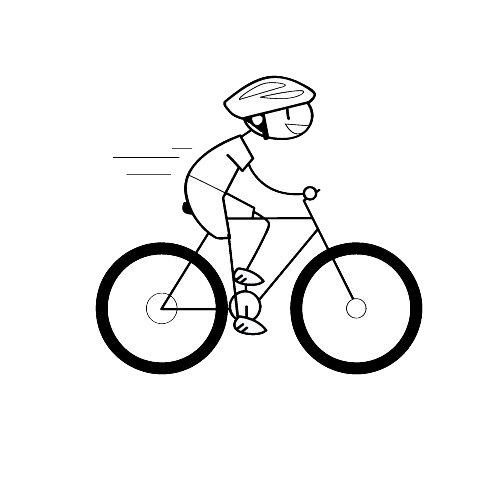
\includegraphics[trim= 0mm 15mm 0mm 5mm,clip,width=0.45\textwidth]{graficos/ciclista.png}
    \caption{Dos imágenes contiguas recortadas para que queden a nivel.}
    \label{fig:3}
\end{figure}

%%%%%%%%%%%%%%%%%%%%%%%%%%%%%%%%%%%%%%%%%%%%
\lipsum

{\bf Final lipsum 4}


\begin{figure}[H] % Requiere paquete float
    \centering
    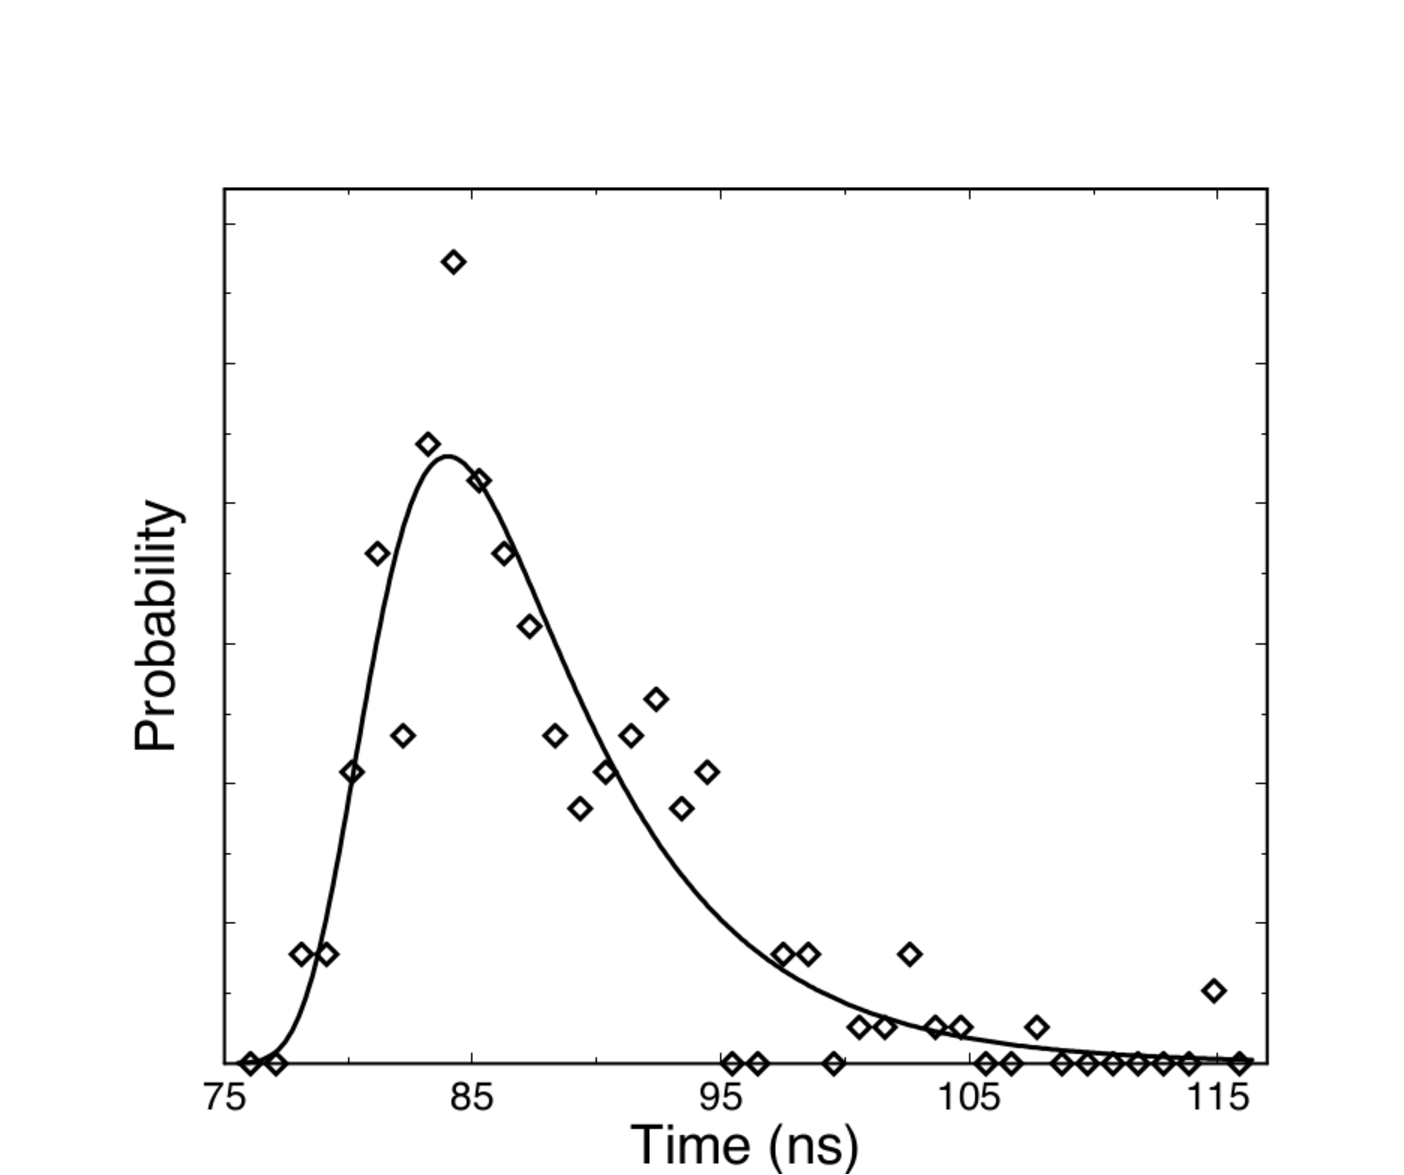
\includegraphics[trim= 0mm 0mm 0mm 30mm,clip,angle=0,width=0.7\textwidth]{graficos/fig_9Vis.pdf}
    \put(-80,150){v=20km/h}
    \put(-100,10){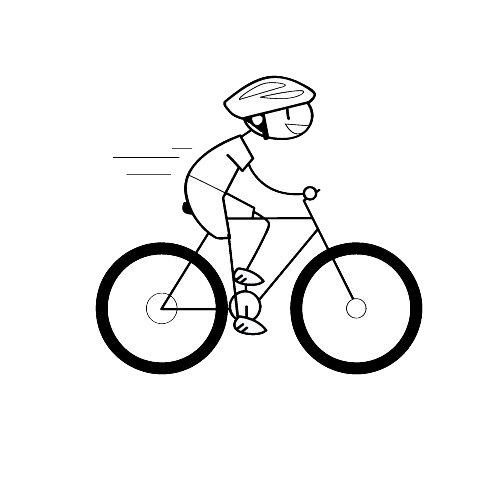
\includegraphics[angle=-7,scale=0.4]{graficos/ciclista.png}}
   % 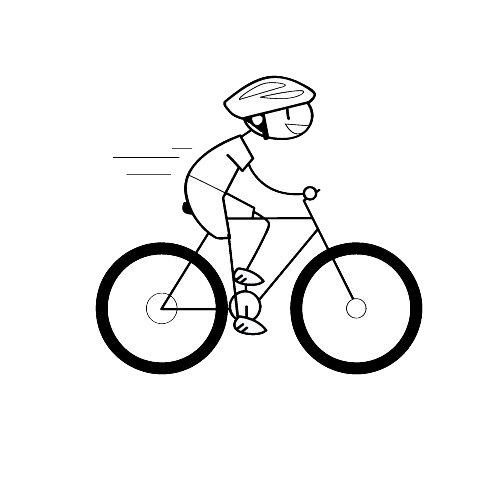
\includegraphics[trim= 0mm 15mm 0mm 5mm,clip,width=0.45\textwidth]{graficos/ciclista.png}
    \caption{Imágen y texto superpuesto. No punto flotante. La responsabilidad de no dejar 
espacios en blanco es nuestra.}
    \label{fig:4}
\end{figure}

%%%%%%%%%%%%%%%%%%%%%%%%%%%%%%%%%%%%%%%%%%%%
\lipsum

{\bf Final lipsum 5}

\begin{wrapfigure}{r}{0.45\textwidth}
 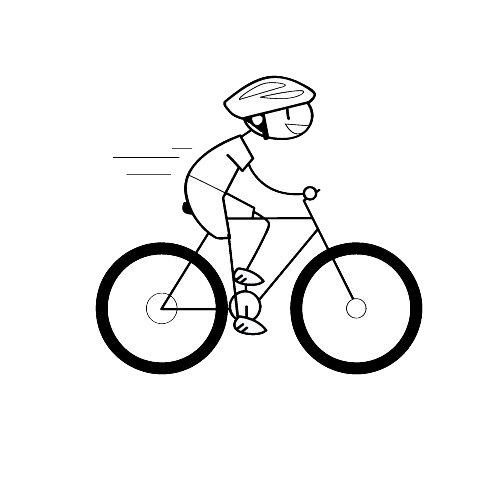
\includegraphics[trim= 0mm 15mm 0mm 8mm,clip,width=0.4\textwidth]{graficos/ciclista.png}
    \caption{Una imagen simple en entorno Wrapfigure}
    \label{Fig:5}
\end{wrapfigure}

%%%%%%%%%%%%%%%%%%%%%%%%%%%%%%%%%%%%%%%%%%%%
\lipsum

{\bf Final lipsum 6}

\begin{figure}[H]  % Requiere paquete float
\centering
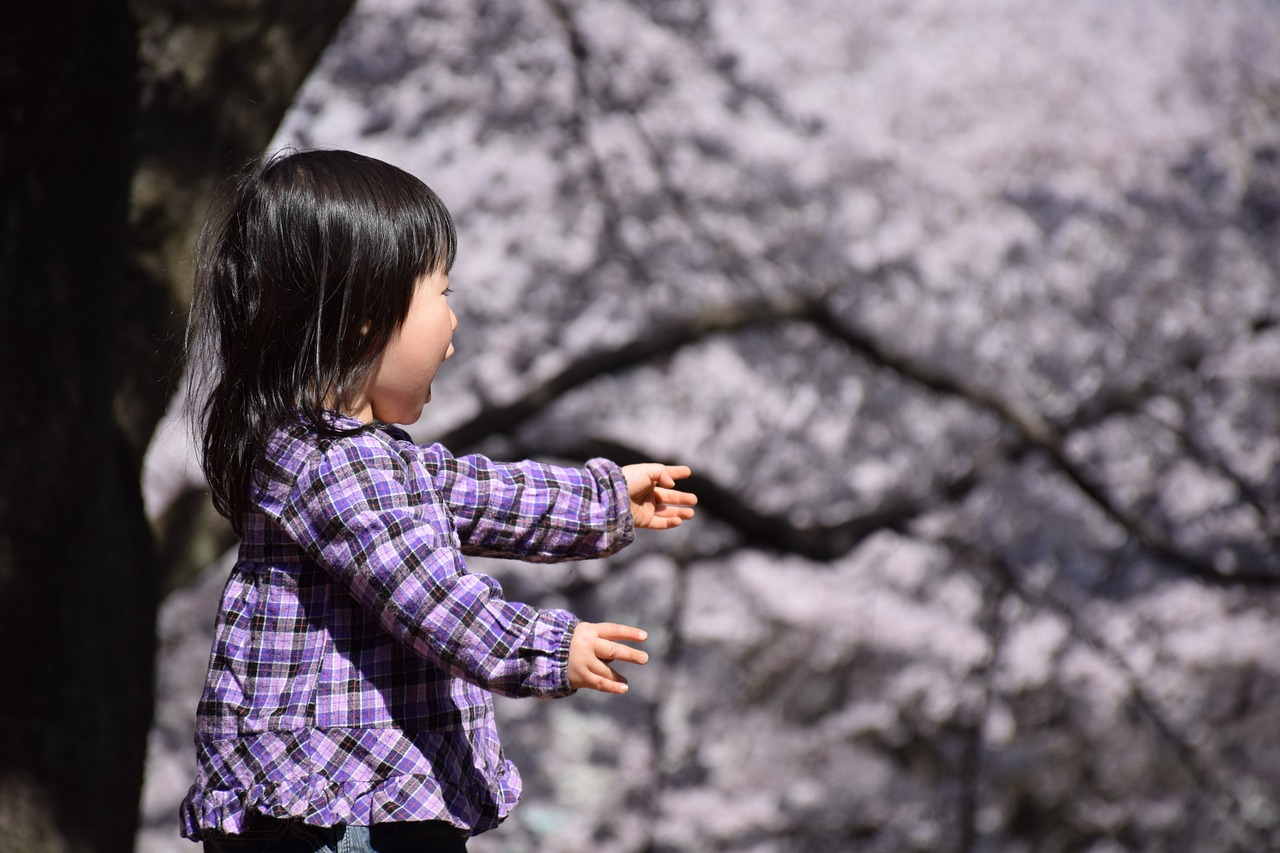
\includegraphics[trim = 50mm 0mm 190mm 40mm, clip,width=5cm]{./graficos/sorpresa}
\hspace{-0.35cm}
\reflectbox{
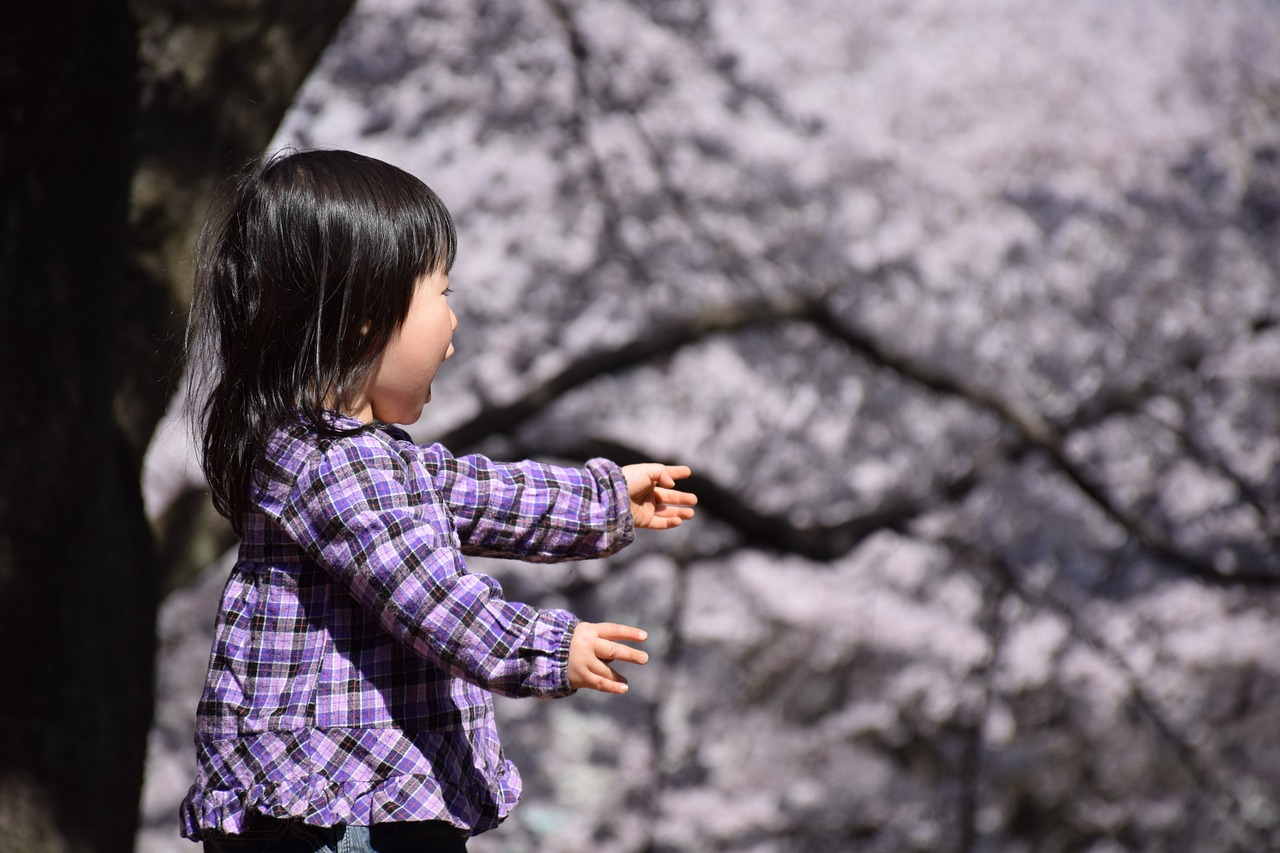
\includegraphics[trim = 50mm 0mm 190mm 40mm, clip,width=5cm]{./graficos/sorpresa}
}
\caption{Montaje con imagen recortada y reflejada. No punto flotante. La responsabilidad de no dejar 
espacios en blanco es nuestra.}
\label{fig:6}
\end{figure}

%%%%%%%%%%%%%%%%%%%%%%%%%%%%%%%%%%%%%%%%%%%%%%%%%%%%%%%%%%%%%

\subsection{Inclusión de páginas pdf}

\includepdf[]{graficos/DeclaraciondeOriginalidadTFG.pdf} % Requiere paquete pdfpages



%%%%%%%%%%%%%%%%%%%%%%%%%%%%%%%%%%%%%%%%%%%%%%%%%%%%%%%%%%%%%

\section{Creación de imágenes con \LaTeX}


\begin{figure}[h]
\begin{tikzpicture}[xscale=1,yscale=1] % Requiere paquete TikZ
\draw[help lines] (0,0) grid (3,3);
\draw[->] (0,0) -- (2,2.5);
\end{tikzpicture}
\hspace{1cm}
\begin{tikzpicture}[xscale=1,yscale=1]
\draw (3,0) -- (1.5,0.5);
\draw[dashed, line width = 1pt, red] (0,0) --(1,2) -- (2,3) -- (1,0);
\end{tikzpicture}
\hspace{1cm}
\begin{tikzpicture}[xscale=0.75,yscale=0.75]
\draw[<->, line width = 1pt] (3,0) --(0,0) -- (0,3);
\draw[->, line width = 0.25pt] (0,0) -- (2,1);
\draw[->,  line width = 0.25pt] (2,1) -- (3,3);
\draw[->, dotted, line width = 0.25pt] (0,0) -- (3,3);
\end{tikzpicture}
\caption{Figuras básicas creadas con TikZ}
\end{figure}


\begin{figure}[h]
\begin{tikzpicture}[xscale=1.5,yscale=1.5]
\draw[<->, line width = 1pt] 
(3.5,0) --(0,0) -- (0,1.5);
\draw [blue, domain=0:pi] 
plot (\x, {sin(\x r)*exp(\x/exp(2*pi))});
\node [below right] at (3.5,0) {$x$};
\node [above left] at (0,1.5) {$y$};
\end{tikzpicture}
\caption{Gráfico generado con TikZ}
\end{figure}


\begin{tikzpicture}[every node/.style={rectangle, fill=blue!20!white}]
\node {Animalia} [sibling distance=6cm]
child {node {Chordata}
	child {node {Vertebrata} [sibling distance=1.5cm]
		child {node {Mammalia}}
		child {node {Aves}}
		}
	}
child {node {Arthoropoda} [sibling distance=4cm]
	child {node {Mandibulata}[sibling distance=2cm]
		child {node {Insecta}}
		child {node {Crustacea}}
		}
	child {node {Chelicerata}
		child {node {Arachnida}}
		}
	};
\end{tikzpicture}

    
%%%%%%%%%%%%%%%%%%%%%%%%%%%%    


% Define block styles
\tikzstyle{decision} = [diamond, draw, fill=blue!20, 
    text width=3.5em, text badly centered, node distance=3cm, inner sep=0pt]
\tikzstyle{block} = [rectangle, draw, fill=blue!20, 
    text width=4em, text centered, rounded corners, minimum height=3em]
\tikzstyle{line} = [draw, -latex']
\tikzstyle{cloud} = [draw, ellipse,fill=red!20, node distance=3cm,
    minimum height=2em]
    


\begin{tikzpicture}[yscale=0.5,node distance = 2cm, auto]
    % Place nodes
    \node [block] (init) {\footnotesize initialize model};
    \node [cloud, left of=init] (expert) {\footnotesize expert};
    \node [cloud, right of=init] (system) {\footnotesize system};
    \node [block, below of=init] (identify) {\footnotesize identify candidate models};
    \node [block, below of=identify] (evaluate) {\footnotesize evaluate candidate models};
    \node [block, left of=evaluate, node distance=3cm] (update) {\footnotesize update model};
    \node [decision, below of=evaluate] (decide) {\footnotesize is best candidate better?};
    \node [block, right of=decide, node distance=3cm] (stop) {\footnotesize stop};
    % Draw edges
    \path [line] (init) -- (identify);
    \path [line] (identify) -- (evaluate);
    \path [line] (evaluate) -- (decide);
    \path [line] (decide) -| node [near start] {yes} (update);
    \path [line] (update) |- (identify);
    \path [line] (decide) -- node {no}(stop);
    \path [line,dashed] (expert) -- (init);
    \path [line,dashed] (system) -- (init);
    \path [line,dashed] (system) |- (evaluate);
\end{tikzpicture}




\end{document}
